\chapter{Data understanding}
\label{ch:data_understanding}

\section{ISIC 2020 challenge dataset}
The ISIC 2020 Challenge Dataset \cite{isic_2020_dataset} is a publicly available collection of dermoscopic images accompanied by detailed metadata. The dataset includes 33,126 annotated training examples and 10,982 test images without annotations. These images depict skin lesions from over 2,000 patients, with both malignant and benign cases represented.

The dataset was curated for the SIIM-ISIC Melanoma Classification Challenge, hosted on Kaggle during the summer of 2020.

A notable limitation of the dataset is its strong tendency to underrepresent darker skin types. This imbalance can be attributed to unequal access to healthcare across populations and societal structures that affect which groups are more likely to be represented. As a result, any solution developed using this dataset is at risk of suffering from skin color bias. While this bias may seem expected given the data, it is a serious challenge from a modeling perspective. If our goal is to develop a truly generalizable solution, we must ensure that it performs equitably across all skin color groups; in other words, that it is fair.

Although the dataset is enriched for melanoma cases and does not reflect the true incidence of melanoma in the general population \cite{isic_2020_dataset}, it also exhibits a significant class imbalance between benign and malignant examples. This presents a major issue, the remedies for which we will discuss in later Chapters \ref{ch:data_preparation}, \ref{ch:modeling}.

The authors of the dataset \cite{isic_2020_dataset} also point out inconsistencies in lighting conditions across images. This variation can lead to inaccurate skin color estimation. If our only goal were to classify malignant lesions without concern for fairness, this might not be a critical issue. However, since we aim to develop a model that is not only high-performing but also fair, our modeling pipeline includes a skin color estimation component, making us directly affected by these inconsistencies.

In our modeling process, we do not use any metadata. We do not incorporate metadata into our knowledge base, nor do we train our models using both images and metadata, and our solution expects only images as input. More details are provided in Chapter~\ref{ch:modeling}.

\section{Skin color estimation}
Skin color is rarely annotated in publicly available dermatological datasets, with only a handful of datasets having labels for either the subject's ethnicity or the actual skin color \cite{skin_color_labels}. Additionally, as skin tone can be difficult to measure and quantify, researchers have not come to a consensus on which scale to use. Research in the makeup industry, for example, saw a need for a fine-grained scale like the L'Oréal skin color map \cite{loreal_chart, accel_fairness}. Medical researchers, on the other hand, needed a scale that reflects the effects ultraviolet light has on different skin tones, so they categorized skin types into the six Fitzpatrick skin phototypes \cite{fitzy} based on how likely each type is to burn or tan when exposed to UV light. Although this scale is completely subjective and is highly biased towards lighter skin tones because of its original application, it is commonly used in research, even when the use case is unrelated with the subject's reactiveness to sunlight. Because of this, we opt to use the individual topology angle (ITA) as a more objective and continuous measure of skin tone. 

\subsection{ITA estimation}
The first step of our data preparation and analysis was to estimate the subject's ITA for each image in the dataset. Following the procedure described in \cite{skin_color_bias_ferit}, we first mask out any pixels that don't contain skin (hair, lesions) and then cluster the remaining pixels to determine the dominant (most populous cluster) skin color in the image. If we represent the resulting color in the CIELAB colorspace, ITA can be estimated from its lightness $L$ and blue-yellow $b$ components. The detailed procedure is visualized in Figure \ref{fig:skin_segmentation} and is also documented in the  \lstinline{notebooks/skin_tone_estimation.ipynb} notebook. In summary, the segmentation procedure is based on image processing and includes increasing contrast with CLAHE, hair removal using DullRazor \cite{dullrazor} and morphologically expanded Otsu thresholding to remove skin pigmentations. 

\begin{figure}[p]
     \centering
     \begin{subfigure}{0.45\textwidth}
         \centering
         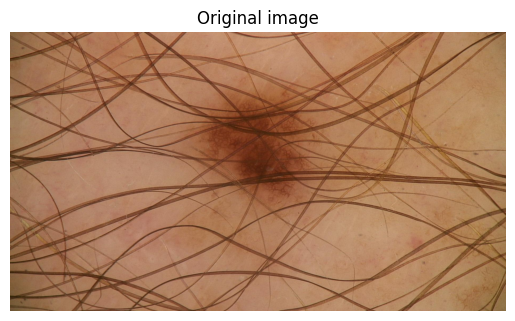
\includegraphics[width=\textwidth]{figures/estimation/estimation_A.png}
         \caption{}
         \label{fig:ss_1}
		 \vspace{0.5em}
     \end{subfigure}
     \hfill
     \begin{subfigure}{0.45\textwidth}
         \centering
         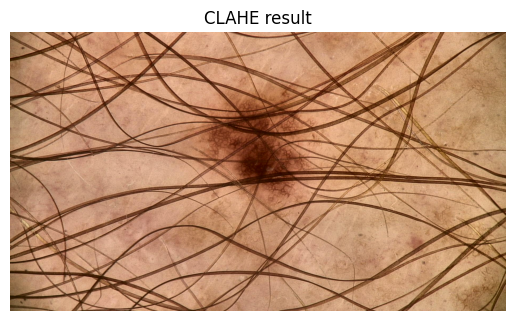
\includegraphics[width=\textwidth]{figures/estimation/estimation_B.png}
         \caption{}
         \label{fig:ss_2}
		\vspace{0.5em}
     \end{subfigure}
    \hfill
     \begin{subfigure}{0.90\textwidth}
         \centering
         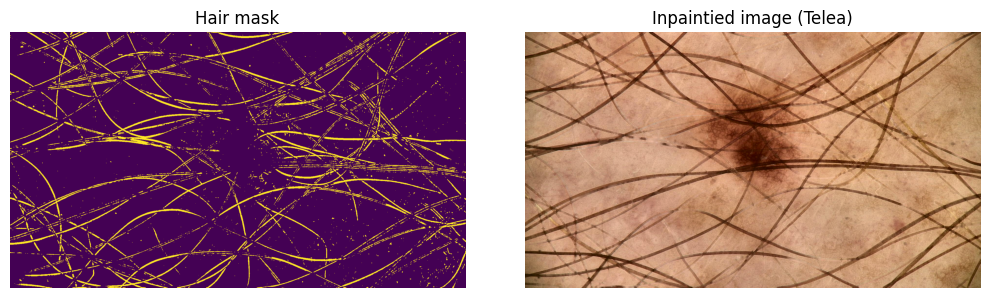
\includegraphics[width=\textwidth]{figures/estimation/estimation_C.png}
         \caption{}
         \label{fig:ss_3}
		 \vspace{0.5em}
     \end{subfigure}
     \hfill
     \begin{subfigure}{0.45\textwidth}
         \centering
         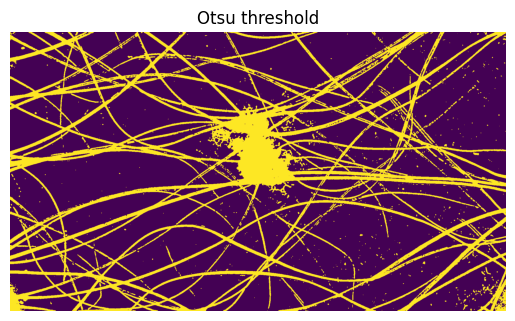
\includegraphics[width=\textwidth]{figures/estimation/estimation_D.png}
         \caption{}
         \label{fig:ss_4}
		 \vspace{0.5em}
     \end{subfigure}
     \hfill
     \begin{subfigure}{0.45\textwidth}
         \centering
         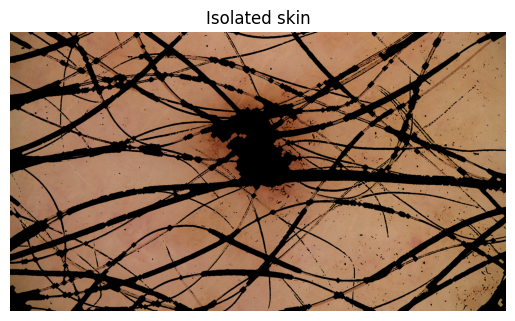
\includegraphics[width=\textwidth]{figures/estimation/estimation_E.png}
         \caption{}
         \label{fig:ss_5}
		 \vspace{0.5em}
     \end{subfigure}
     \hfill
     \begin{subfigure}{0.90\textwidth}
         \centering
         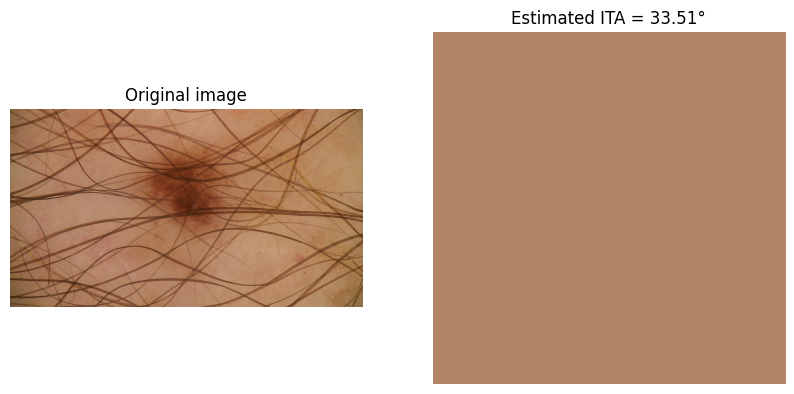
\includegraphics[width=\textwidth]{figures/estimation/estimation_F.png}
         \caption{}
         \label{fig:ss_5}
		 \vspace{0.5em}
     \end{subfigure}
     \hfill
	\caption{Individual steps and results of the skin segmentation and color estimation procedure.}
	\label{fig:skin_segmentation}
\end{figure}

\begin{table}[]
\centering
\caption{Skin groups based on individual topology angle values from \cite{chardon}}
\label{tab:ita_ranges}
\begin{tabular}{lr}
\toprule
\textbf{ITA skin group} & \textbf{ITA range}  \\ \midrule
Very light              & $ > 55 $              \\
Light                   & $ \left<41, 55\right]$ \\
Intermediate            & $ \left<28, 41\right]$ \\
Tan                     & $ \left<-30.10\right]$ \\
Brown                   & $ \left<10, 28\right]$ \\
Dark                    & $ \le -30 $           \\ \bottomrule
\end{tabular}
\end{table}


Continuous skin tone labels like ITA enable us to test for correlations with continuous outputs of our model (e.g. prosterior probabilities of the malignant class) and in general contain more information than discrete skin tone types. Despite this, the task at hand is a classification one and our target variables are discrete (benign, malignant), so most fairness assessment techniques will require our data to be grouped based on skin tone. Because of this we discretize ITA into the six groups proposed in \cite{chardon}, shown in Table \ref{tab:ita_ranges}. As argued by \cite{letter_ita_fp} and as we previously hinted, we emphasize that these groups are not equivalent to the six Fitzpatrick phototypes which are more subjective and based on sun reactiveness of the subject's skin.

Figure \ref{fig:kde} shows the KDE plots of estimated ITA values for malignant and benign classes in the available dataset (aggregated training and validation sets of ISIC2020). It is evident that the dataset is biased towards lighter skin tones, especially in the benign case. The distribution of malignant ITAs is slightly wider, and its mean is shifted slightly more towards darker skin tones. Looking at skin color distributions with respect to the discrete ITA groups (Figure \ref{fig:histograms}), we notice that our dataset has no samples in the dark group, and that there are only two malignant samples in the brown group. These histograms show that, in addition to being imbalanced with respect to skin tone, our dataset is highly skewed towards the benign class. Most notably, malignant samples only make up $1.3 \%$ of the intermediate skin tone group. This is not surprising, as positive samples are bound to come up less often than negative ones when collecting dermoscopic or medical data. We see that our dataset is imbalanced in two orthogonal directions: with respect to skin color and malignancy. This is important to keep in mind in further analysis to be able to select appropriate classification models and methods.

\begin{figure}[htpb]
     \centering
     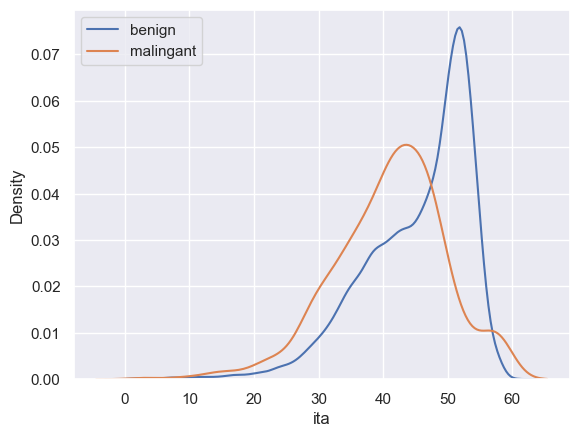
\includegraphics[width=0.8\textwidth]{figures/eda/kde.png}
     \caption{Per class individual topogy angle distributions in the available data.}
     \label{fig:kde}
\end{figure}
\begin{figure}[htpb]
     \centering
     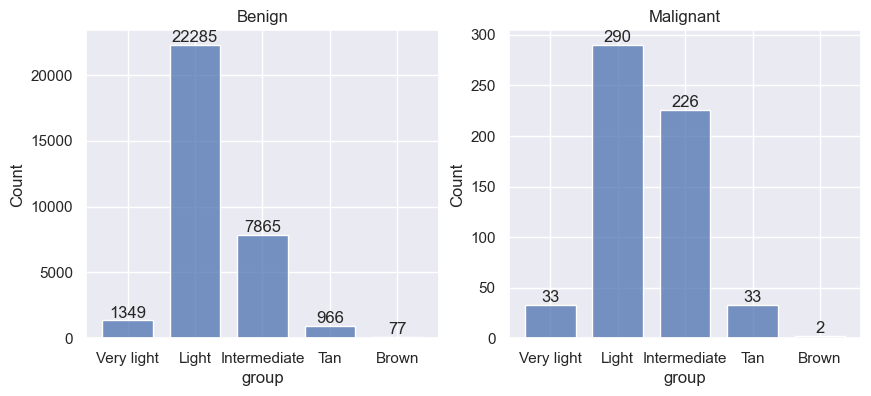
\includegraphics[width=\textwidth]{figures/eda/histograms.png}
     \caption{Number of images in each skin color group for benign and malignant classes.}
     \label{fig:histograms}
 \end{figure}

\subsection{Estimation error checking}
Because we are doing automatic skin color estimation, we want to manually check for errors in the estimation results, and make sure that the estimated skin tones match our expectations for each group. Appendix \ref{ap:skin_color} shows 64 images from each skin color group, along with the estimated ITA values and corresponding dominant skin colors. With lighter skin tones and small lesions, the estimation appears to work correctly, and there is no need for corrections. We find that a lot of images which are classified as brown are heavily cropped and only show the lesion, with the surrounding skin being barely visible. In some of those cases we see that the skin color is actually much lighter than the predicted dominant one, and that the estimation was incorrect. 

Focusing only on the malignant samples in the brown and tan groups (Figure \ref{fig:ita_errors}), five mislabelled samples (marked in red) can be seen. These labels were corrected by taking the average RGB value in a 5x5 px area that was manually selected to only contain skin, and converting them to the CIELAB colorspace to calculate the corresponding ITA. The corrected skin tone labels are compared to the automatically estimated ones in Figure \ref{fig:ita_fixed}.

\begin{figure}[htpb]
     \centering
     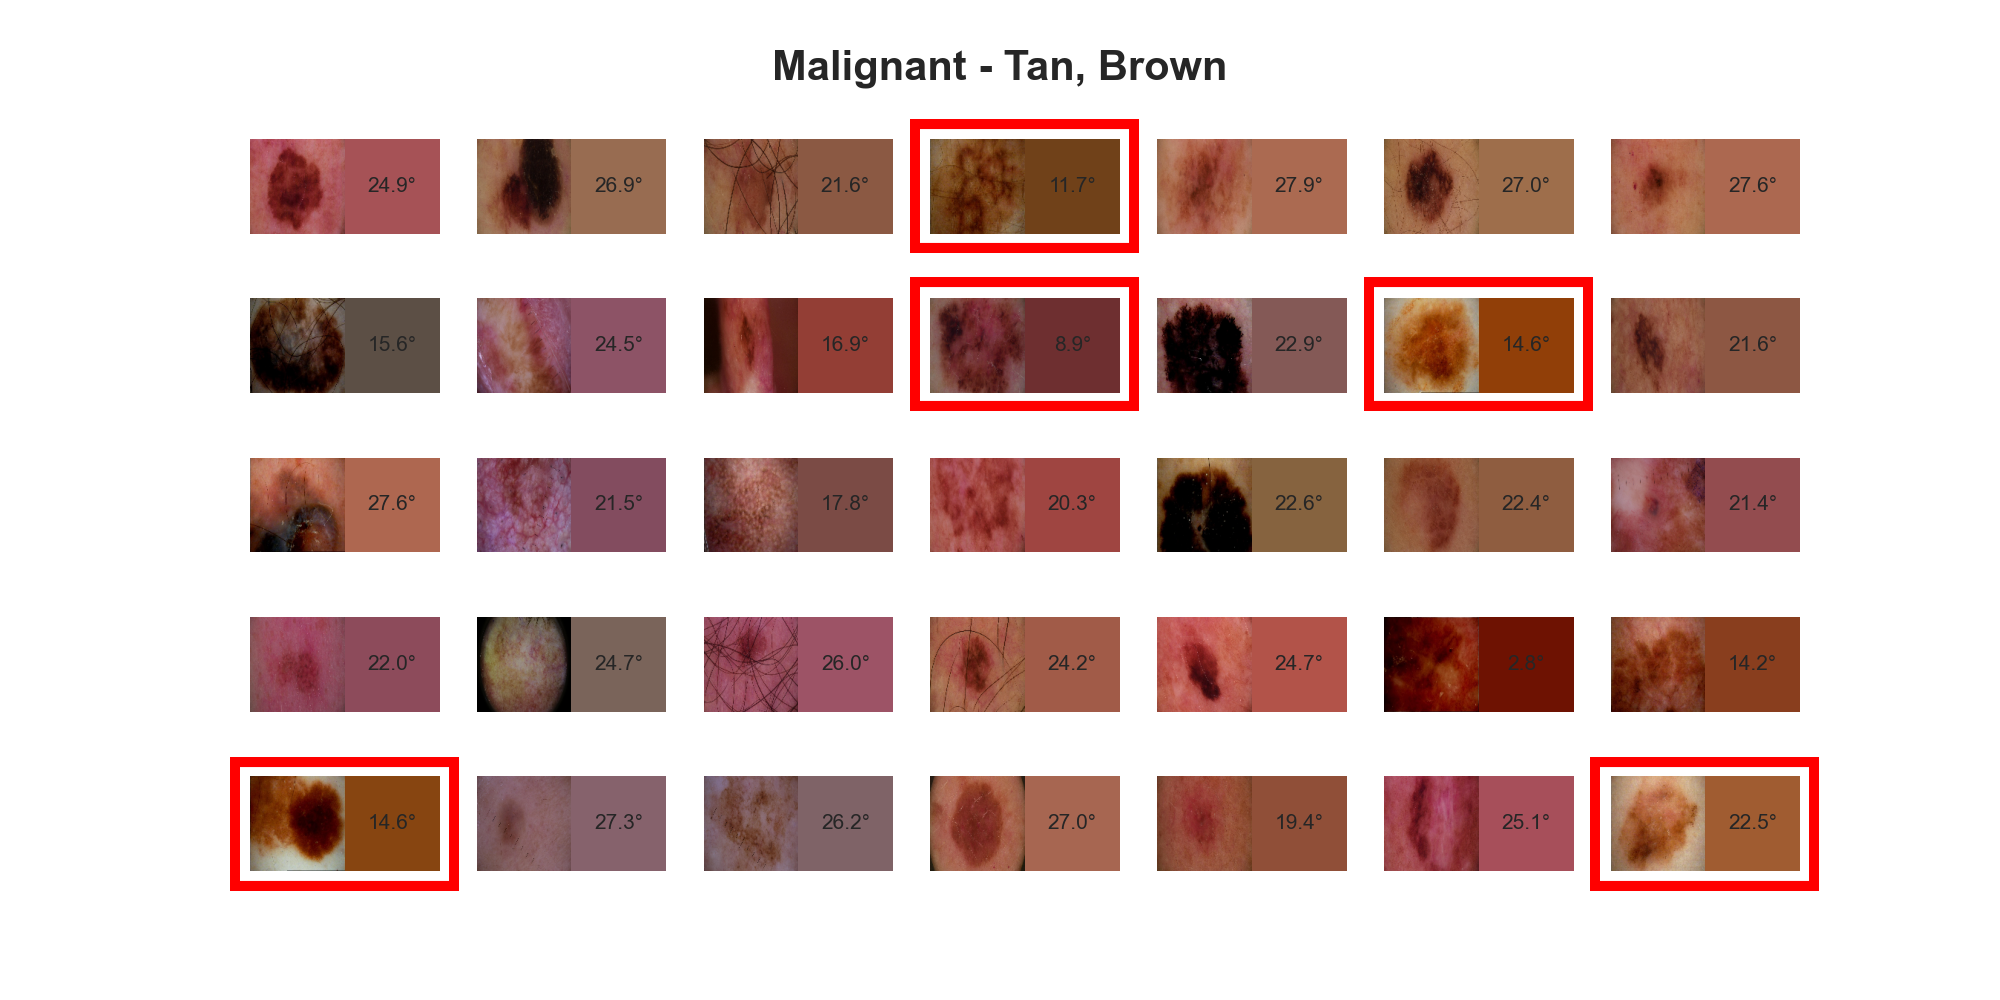
\includegraphics[width=0.99\textwidth]{figures/eda/Malignant, Tan_Brown, errors.png}
     \caption{All malignant samples labeled as tan or brown. Images with incorrect ITA estimates are marked with a red rectangle.}
     \label{fig:ita_errors}
\end{figure}

\begin{figure}[htpb]
     \centering
     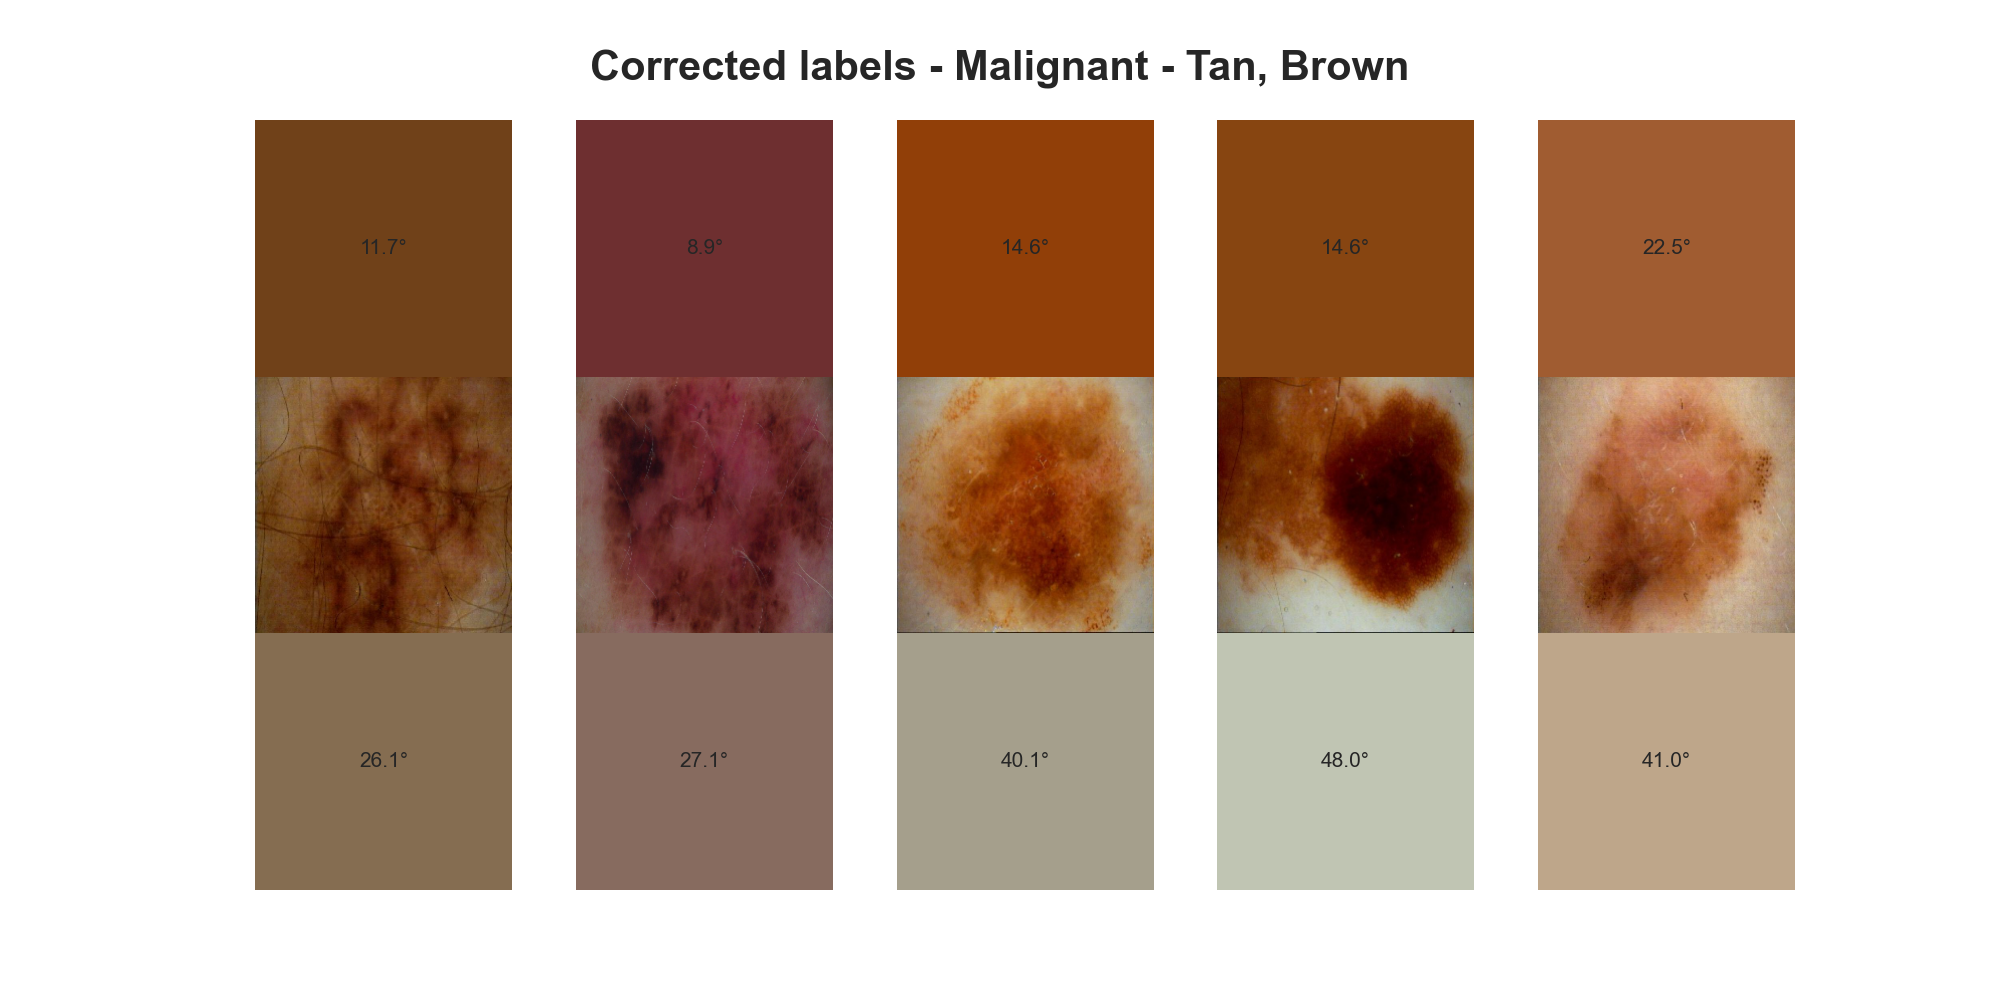
\includegraphics[width=0.99\textwidth]{figures/eda/Corrected - Malignant, Tan_Brown.png}
     \caption{Malignant samples (middle row) from the brown and tan groups with incorrectly estimated ITA values (top row), and manually corrected labels (bottom row).}
     \label{fig:ita_fixed}
\end{figure}

\subsection{Image artefacts}
Artefacts like surgical pen markings, hair and dark corners are also clearly visible in Figure \ref{fig:skin_colors_1}. This, along with physical rulers, pockets of air in the applied immersion fluid, dermoscope measurement overlays etc., are widespread throughout dermoscopic datasets \cite{isic_recommendations}. It's important to be aware of them, because visual artefacts can easily introduce bias to our models and decrease generalization performance, e.g. if the model learns to correlate the presence of pen markings with the malignant class. 
